\newpage
\section{Setting up your workspace}
\genHeader

Before starting any TGG transformation, you'll need to have the separate source and target metamodels already prepared. In our case, these will be
\texttt{LeitnersLearningBox} and a new \texttt{DictionaryLanguage}. Don't worry - we have created this for you to import into your workspace. If you haven't
completed the previous parts in the handbook series, work through Section~\ref{sec:loadSourceMeta} to load a pre prepared \texttt{LeitnersLearningBox}
metamodel into your workspace. If your source metamodel is ready to go however, skip ahead to  either \texttt{\hyperlink{sec:multiEAP}{Section 2.2 (Visual)}}
or \texttt{\hyperlink{sec:multiMOSL}{Section 2.3 (Textual)}}.


% --- NEW USER INSTRUCTIONS
\subsection{Starting Fresh}
\label{sec:loadSourceMeta}
\begin{itemize}

\item[$\blacktriangleright$] Press the \texttt{new} button on the toolbar and navigate to ``Examples/eMoflon Handbook Examples/''
(Fig.~\ref{fig:downPartIV}).  We have created two cheat packages based on eMolfon's two specification types. For a brief discussion on the differences between
the two, refer to Part I, Section I. They are both completed with all objects, references, and implemented SDMs.

\begin{figure}[htbp]
\begin{center}
  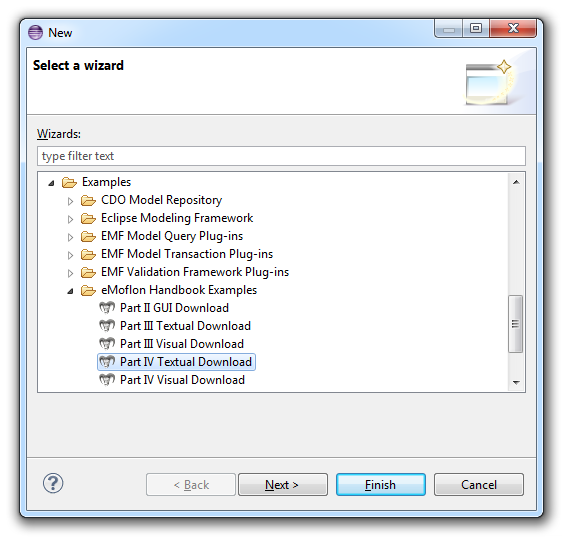
\includegraphics[width=0.8\textwidth]{eclipse_downloadWizardPartIV}
  \caption{Use the wizard to download your cheat package}
  \label{fig:downPartIV}
\end{center}
\end{figure}

\item[$\blacktriangleright$] After loading, if your package explorer does not resemble ours in Fig.~\ref{fig:workingSets} with at least two
distinct nodes, select the small, downward facing arrow in the corner of the module window. Choose ``Working Sets/Top Level Elements.'' To review how these
nodes are used to structure the workspace in Eclipse, check out Part I, Section 4.

\vspace{0.5cm}

% Forced placement so it would co-operate
\begin{figure}[h!]
	\centering
  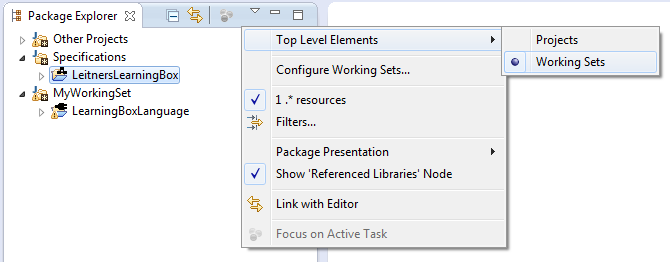
\includegraphics[width=0.9\textwidth]{eclipse_workingSets}
	\caption{Setting your Package Explorer}
	\label{fig:workingSets}
\end{figure}

\vspace{0.5cm}

At this point we recommend reading the introduction to Part II for a detailed overview of \texttt{LeitnersLearningBox}, its purpose and goals, and how
\texttt{card}s and \texttt{FastCards} are moved between each \texttt{partition}. It should only take a minute or two, and the background information may help
you better understand the reasoning behind some steps in this part as we continue to build on the idea.

\end{itemize}

\jumpDual{multiEAP}{multiMOSL}

% Instructions for loading target model
\newpage
\hypertarget{multiEAP}{}
\subsection{Importing and working with multiple EAPs}
\visHeader

Please note that the following instructions on how to properly export and import Enterprise Architect (EA) files are \emph{not} an eMoflon-exclusive feature.
We have included them here as part of our handbook as getting this right is crucial for working with eMoflon, especially when working with TGGs. The main
problem is that, as far as we know, EA does not (yet) support referencing model elements in one EAP from another, completely different EAP. This means that all
required metamodels have to first be merged in the same EAP before such references can be specified (as required for TGGs).

\begin{itemize}

\item[$\blacktriangleright$] Press the \texttt{new} button in the Eclipse toolbar and navigate to ``Examples/eMoflon Handbook Examples/''
(Fig.~\ref{eclipse:dictionaryDownloadWizard}). Find and select \texttt{Part IV Visual Dictionary Language} to copy a new \texttt{Dict\-ion\-ary\-Lang\-uage}
metamodel project into your workspace.

\vspace{0.5cm}

% Image stored in ../1_gettingStarted/textImportImages/  (repeated image)
\begin{figure}[htbp]
\begin{center}
  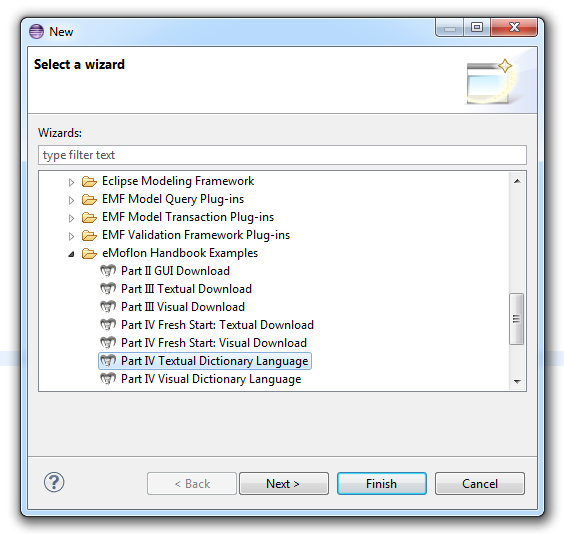
\includegraphics[width=0.8\textwidth]{eclipse_part4DictionaryLanguageDownload}
  \caption{Get the visual \texttt{DictionaryLanguage} metamodel}
  \label{eclipse:dictionaryDownloadWizard}
\end{center}
\end{figure}

\item[$\blacktriangleright$] If successful, your workspace should resemble Fig.~\ref{eclipse:loadedDictionaryEAP}. Double-click
\texttt{Dictionary.eap} to open it in EA.

\newpage

\begin{figure}[htbp]
\begin{center}
  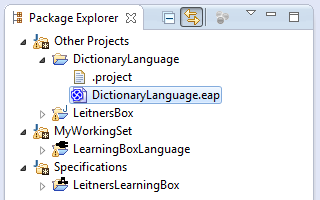
\includegraphics[width=0.5\textwidth]{eclipse_loadedDictionaryEAP}
  \caption{\texttt{Dictionary} metamodel successfully copied into the workspace}
  \label{eclipse:loadedDictionaryEAP}
\end{center}
\end{figure}

\item[$\blacktriangleright$] The file's project browser should resemble Fig.~\ref{ea:dictionaryLangStart}. Feel free to inspect the main
\texttt{DictionaryLanguage} diagram until you're familiar with the metamodel. Our work will be focused on the \texttt{Dictionary} and \texttt{Entry} classes.
You'll be able to see that dictionaries can be assigned unique \texttt{EString title}s, and each entry will have some sort of \texttt{content} matched with one
of three difficulty \texttt{level}s.

\vspace{0.5cm}

\begin{figure}[htbp]
\begin{center}
  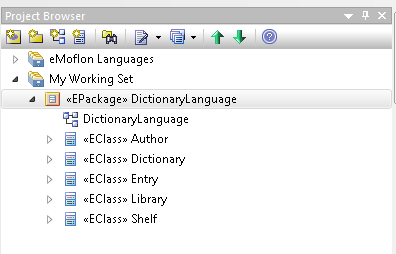
\includegraphics[width=0.4\textwidth]{ea_dictLangProBrowser}
  \caption{The \texttt{DictionaryLanguage} metamodel structure}
  \label{ea:dictionaryLangStart}
\end{center}
\end{figure}

\item[$\blacktriangleright$] It should be said that while you are able to simply copy and paste packages between multiple EAPs (i.e., copy
\texttt{<<E\-Pack\-age>>Dict\-ion\-ary\-Lang\-uage} into the \texttt{MyWorkingSet} root note of your source metamodel), if any of the copied packages have
dependencies on other packages, it cannot be done so easily. All links would be destroyed! 

\clearpage

\item[$\blacktriangleright$] Therefore, to properly migrate the \texttt{DictionaryLanguage} package, right-click on the EPackage root, navigate to
``Import/Export" and select \texttt{Export Model to XMI\ldots} (Fig.~\ref{ea:contextExport}). Alternatively, you can select the root in the project browser and
press \texttt{Ctrl + Alt + E}.

\vspace{0.5cm}

\begin{figure}[htbp]
\begin{center}
  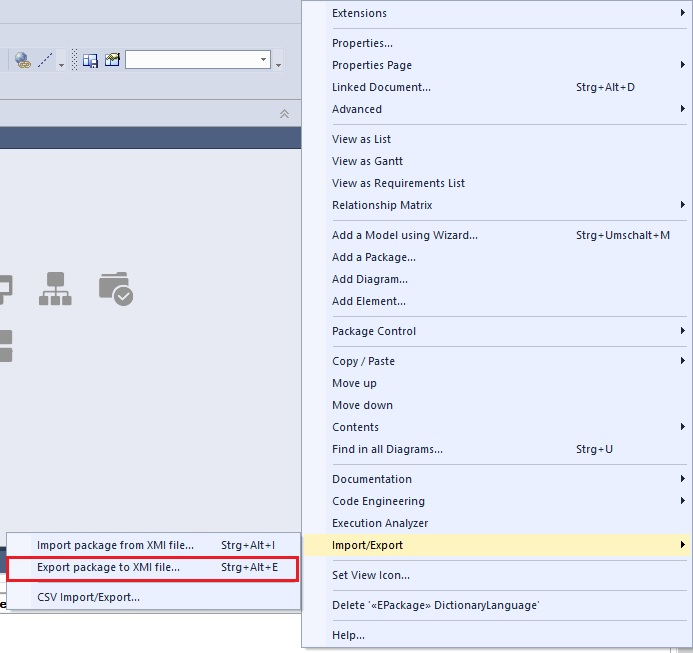
\includegraphics[width=\textwidth]{ea_contextExport}
  \caption{Starting the export process in EA}
  \label{ea:contextExport}
\end{center}
\end{figure}

\item[$\blacktriangleright$] Switch the export type to \texttt{XMI 2.1} in the dialogue and save the file somewhere easily accessible. Press export, and close
the window once the small green bar appears (Fig.~\ref{ea:export}).

\begin{figure}[htbp]
\begin{center}
  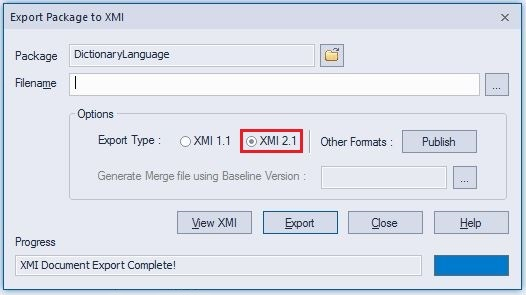
\includegraphics[width=0.9\textwidth]{ea_dialogueExport}
  \caption{Exporting the metamodel to a file}
  \label{ea:export}
\end{center}
\end{figure}

\item[$\blacktriangleright$] Go back to Eclipse and open \texttt{LeitnersLearningBox.eap}. Right-click on \texttt{MyWorkingSet} and navigate to ``Import
Model from XMI\ldots''

\item[$\blacktriangleright$] Find the \texttt{.xmi} file you just saved and press \texttt{import}. Press \texttt{OK} in the confirmation dialogue; Your project
browser should now resemble Fig.~\ref{ea:importProBrowser}, with both metamodels in the same working set, in the same EAP.

\begin{figure}[htbp]
\begin{center}
  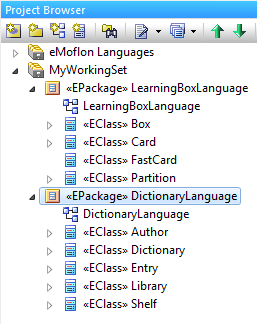
\includegraphics[width=0.5\textwidth]{ea_loadedDictionaryMetamodel}
  \caption{The TGG metamodels successfully included in one EAP}
  \label{ea:importProBrowser}
\end{center}
\end{figure}

\clearpage

\item[$\blacktriangleright$] Confirm the import by validating\footnote{To review the details of how to use the eMoflon control panel, read Section 2.8 from
Part II} (Fig.~\ref{ea:importValidationWindow}) and exporting the dual-metamodel project to Eclipse, refreshing \texttt{LeitnersLearningBox} to rebuild your workspace. 

\vspace{0.5cm}

\begin{figure}[htbp]
\begin{center}
  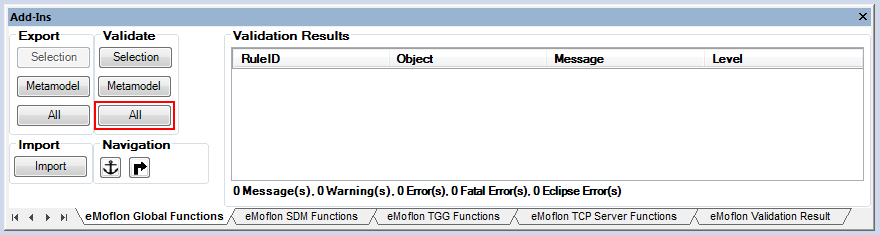
\includegraphics[width=\textwidth]{ea_importValidationWindow}
  \caption{No validation errors for \texttt{LeitnersLearningBox}}
  \label{ea:importValidationWindow}
\end{center}
\end{figure}

\vspace{0.5cm}

\item[$\blacktriangleright$] That's it! You now have the second metamodel for your transformation, and are ready to start specifying your TGG rules.

\jumpSingle{TGGSchema}

\end{itemize}


\newpage
\hypertarget{multiMOSL}{}
\subsection{Working with multple MOSL projects}
\texHeader

% Eclipse import instructions; all unconfirmed.
\begin{itemize}

\item[$\blacktriangleright$] Confirm your source metamodel \texttt{LeitnersLearningBox}, is in the current workspace prepared and right-click on
\texttt{MyWorkingSet}. Select \texttt{Import\ldots} from the context menu (Fig.~\ref{fig:eclipseContextImport}).

\vspace{0.25cm}

\begin{figure}[htbp]
\begin{center}
  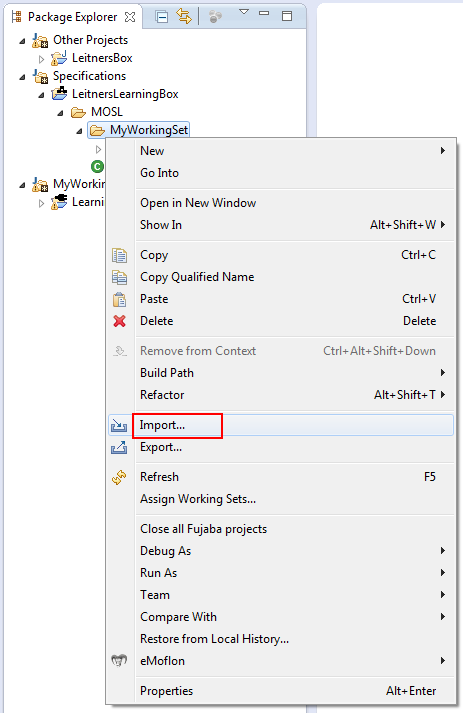
\includegraphics[width=0.6\textwidth]{eclipse_contextImport}
  \caption{caption}
  \label{fig:eclipseContextImport}
\end{center}
\end{figure}

\item[$\blacktriangleright$] In the first dialogue, set your import source by navigating to ``General/File System.'' This is the appropriate choice since
we want to import the entire directory structure of the target metamodel, not a pre existing project.

\item[$\blacktriangleright$] Press \texttt{Browse\ldots} and navigate to the folder where you extracted the contents of the \texttt{Part4.zip} download file
which included this document (Fig.~\ref{fig:importFileSys}). Press \texttt{Select All} to ensure you're importing all the necessary MOSL files for your TGG
target metamodel. Affirm and close the dialogue by pressing \texttt{Finish}.

\newpage

\begin{figure}[htbp]
\begin{center}
  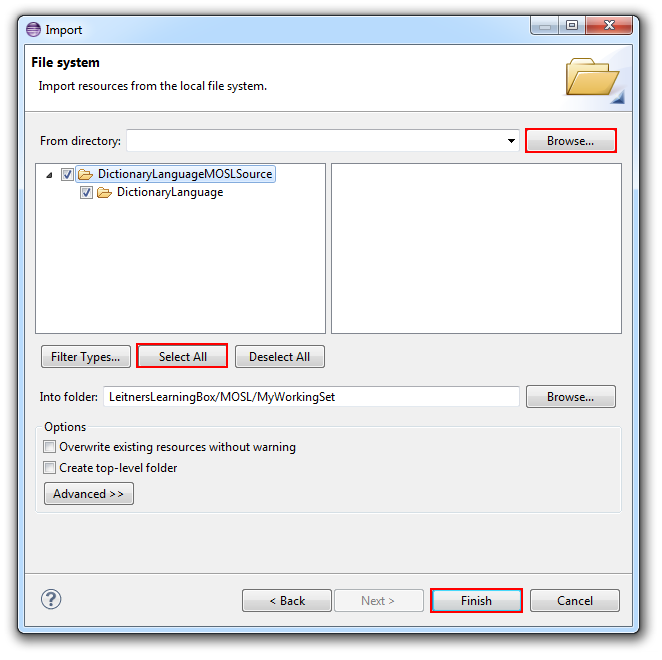
\includegraphics[width=0.8\textwidth]{eclipse_importDialogue}
  \caption{caption}
  \label{fig:importFileSys}
\end{center}
\end{figure}

\item[$\blacktriangleright$] With your project now loaded, navigate to ``Build (Without Cleaning)'' on the toolbar to build both metamodels. Confirm with
Fig.~\ref{fig:bothmetamodelstructures} that your MOSL directory is now populated with both metamodels, and notice that a second \texttt{Dictionary\-Language}
folder appeared under the same node as the \texttt{LearningBoxLanguage} repository project. If you expand this folder, you'll be able to see that it has
similar generated code for the imported metamodel.

\begin{figure}[htbp]
\begin{center}
  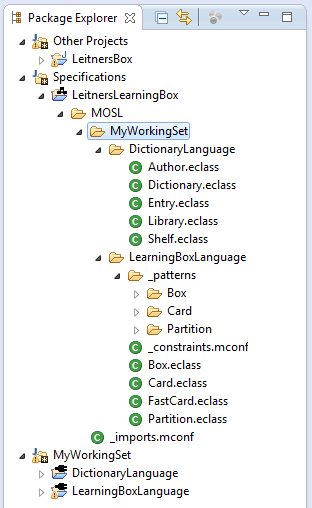
\includegraphics[width=0.5\textwidth]{eclipse_metamodelStructures}
  \caption{Fully loaded dual-metamodel structure}
  \label{fig:bothmetamodelstructures}
\end{center}
\end{figure}

\item[$\blacktriangleright$] Great work -- You're now ready to start using your metamodels in a TGG transformation! If you've just joined us and are interested
in the eMoflon project structure, or curious as to how Java code is generated, we invite you to read Section 4.2 from Part I. Otherwise, continue to the next section to begin
building your TGG Schema. 

\end{itemize}

